\documentclass[a4paper,oneside,12pt]{article}

\usepackage[slovene]{babel}    % slovenian language and hyphenation
\usepackage[utf8]{inputenc}    % make čšž work on input
\usepackage[T1]{fontenc}       % make čšž work on output
\usepackage[reqno]{amsmath}    % basic ams math environments and symbols
\usepackage{amssymb,amsthm}    % ams symbols and theorems
\usepackage{mathtools}         % extends ams with arrows and stuff
\usepackage{url}               % \url and \href for links
\usepackage{icomma}            % make comma a thousands separator with correct spacing
\usepackage{units}             % \unit[1]{m} and unitfrac
\usepackage{enumerate}         % enumerate style
\usepackage{array}             % mutirow
\usepackage[usenames]{color}   % colors with names
\usepackage{graphicx}          % images

\usepackage[bookmarks, colorlinks=true, linkcolor=black, anchorcolor=black,
  citecolor=black, filecolor=black, menucolor=black, runcolor=black,
  urlcolor=black, pdfencoding=unicode]{hyperref}  % clickable references, pdf toc
\usepackage[
  paper=a4paper,
  top=2.5cm,
  bottom=2.5cm,
  left=2.5cm,
  right=2.5cm
% textheight=24cm,
]{geometry}  % page geomerty

\newcommand{\R}{\ensuremath{\mathbb{R}}}
\newcommand{\N}{\ensuremath{\mathbb{N}}}
\newcommand{\Z}{\ensuremath{\mathbb{Z}}}
\renewcommand{\C}{\ensuremath{\mathbb{C}}}
\newcommand{\Q}{\ensuremath{\mathbb{Q}}}
\newcommand{\T}{\ensuremath{\mathsf{T}}}


\newcommand{\Title}{}
\newcommand{\Author}{Jure Slak}
\title{\Title}
\author{\Author}
\date{\today}
\hypersetup{pdftitle={\Title}, pdfauthor={\Author}, pdfcreator={\Author},
            pdfproducer={\Author}, pdfsubject={}, pdfkeywords={}}  % setup pdf metadata

% \pagestyle{empty}              % vse strani prazne
% \setlength{\parindent}{0pt}    % zamik vsakega odstavka
% \setlength{\parskip}{10pt}     % prazen prostor po odstavku
\setlength{\overfullrule}{30pt}  % oznaci predlogo vrstico z veliko črnine

\usepackage{algorithm}
\usepackage{algpseudocode}

\floatname{algorithm}{Algoritem}
\renewcommand{\listalgorithmname}{Kazalo algoritmov}
\algnewcommand\algorithmicto{\textbf{to}}
\algnewcommand\algorithmicin{\textbf{in}}
\algnewcommand\algorithmicforeach{\textbf{for each}}
\algrenewtext{For}[3]{\algorithmicfor\ #1 $\gets$ #2\ \algorithmicto\ #3\ \algorithmicdo}
\algdef{S}[FOR]{ForEach}[2]{\algorithmicforeach\ #1\ \algorithmicin\ #2\ \algorithmicdo}

\usepackage[all]{xy}
\usepackage{minted}
\usepackage{tikz}
\usetikzlibrary{decorations.pathreplacing}

\begin{document}

\section{BibTeX}
Vključevanje literature je lahko: potrebujete le dva ukaza:
\verb|\bibliography{file}| in \verb|\bibliographystyle{file}|.
Citirate kot običajno s \verb|\cite|.

\section{Pisanje algoritmov}
Za pisanje algoritmov sta na voljo okolji \texttt{algorithm} in
\texttt{algorithmic} iz paketov \texttt{algorithm} in \texttt{algorithmix}, ki
sodelujeta podobno kot \texttt{table} in \texttt{tabular}. Algoritmi plavajo
med tekstom, enako kot slike in tabele, nanje se lahko tudi sklicujemo, kot
prikazano v izvorni kodi in v algoritmu~\ref{alg:metoda}. Sklicujemo se lahko
tudi na pomembne vrstice, npr.\ na vrstico~\ref{alg:pomembna-vrstica}, ki
predstavlja glavni del algoritma. Za primer pisanja algoritma se posvetujte s
primerom v tem dokumentu, za bolj napredne primere uporabe, kot na primer
razbijanje algoritma na več kosov, pa z (precej razumljivo) uradno
dokumentacijo\footnote{\url{http://tug.ctan.org/macros/latex/contrib/algorithmicx/algorithmicx.pdf}}.


\begin{algorithm}[ht]
  \caption{Opis, ki ima enako funkcionalnost kot opis pod sliko.}
  \label{alg:metoda}
  \raggedright
  \textbf{Vhod:} Števili $n, m \in \N, n > m$. \\
  \textbf{Izhod:} Decimalno število $x$, ki aproksimira rešitev enačbe $n x = m$.
  \begin{algorithmic}[1]
    \Function{reši}{$n$, $m$} \Comment{Vsi vhodni parametri morajo biti opisani.}
    \State $a \gets [\,]$ \Comment{Spremenljivka $a$ naj postane prazna kopica.}
    \For{$i$}{$1$}{$n$}
    \If{$i \operatorname{mod} 7 = 5$}
    \State \Call{heapop}{$a$}
    \ElsIf{$i < 5$}
    \State \Call{heappush}{$a, \frac{i+12}{7} + \pi$} \Comment{Lahko uporabljamo matematiko.}
    \Else
    \State \Call{heappush}{$a, i$}
    \EndIf
    \EndFor
    \Statex  \Comment{Prazna vrstica}
    \State $x \gets 0$  \Comment{To je primer komentarja.}
    \ForEach{e}{a}
    \State $x \gets 1 + \sqrt[e]{x}$
    \EndFor
    \While{$|x| > \varepsilon$}
    \State $x \gets x / 2$
    \EndWhile
    \State $x \gets m / n$ \label{alg:pomembna-vrstica}
    \State \Return $x$  \Comment{Vsi izhodni parametri morajo biti opisani nad algoritmom.}
    \EndFunction
  \end{algorithmic}
\end{algorithm}

\section{Izvorna koda}
Paket \verb|minted|\footnote{\url{http://ctan.ijs.si/tex-archive/macros/latex/contrib/minted/minted.pdf}}. Potrebuje program \verb|pygmentize| za barvanje kode.

\begin{minted}[linenos]{python}
  a = input()
  for i in range(10):
      print(i)
\end{minted}

Lahko tudi iz datoteke ali inline.

\section{Diagrami}

Uporabljamo paket \verb|xy|\footnote{\url{https://en.wikibooks.org/wiki/LaTeX/Xy-pic}}.
User guide: {\small \url{http://ctan.ijs.si/tex-archive/macros/generic/diagrams/xypic/doc/xyguide.pdf}}

\[
\xymatrix{
 a \ar[r] \ar[d] \ar[dr]_{x}& b \ar[d] \\ c \ar[r] & d
}
\]

\section{MakeIndex}
Izdelava stvarnih kazal.

\section{Tikz}
Risanje risbic. Navodila: \url{https://www.bu.edu/math/files/2013/08/tikzpgfmanual.pdf}.



% Define style for nodes
\tikzstyle{every node}=[circle, draw, fill=black!10,
inner sep=0pt, minimum width=4pt]

Preproste oblike; lahko kar tako, 
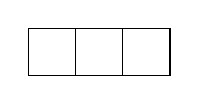
\begin{tikzpicture}[scale=0.6]				
\draw (16,0) -- (19, 0) -- (19,1) -- (16,1) -- (16,0);
\draw (17,0) -- (17,1);
\draw (18,0) -- (18,1) -- (19,1);
\end{tikzpicture}

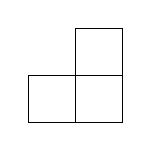
\begin{tikzpicture}[scale=0.6]				
\draw (16,0) -- (18, 0) -- (18,2) -- (17,2) -- (17,1) -- (16,1) -- (16,0);
\draw (17,1) -- (18,1);
\draw (17,0) -- (17,1);
\end{tikzpicture}
lahko pa v okolju za sliko.
\begin{figure}[ht!]
	\begin{center}
		\begin{tikzpicture}[scale=0.8]
		
		\draw (0,0) -- (2,0) -- (2,2) -- (0,2) -- (0,0);
		\draw (0,1) -- (2,1);
		\draw (1,0) -- (1,2);
		
		\draw (4,0) -- (6,0) -- (6,1) -- (5,1) -- (5,2) -- (3,2) -- (3,1) -- (4,1) -- (4,0);
		\draw (5,0) -- (5,1) -- (4,1) -- (4,2);
		
		\draw (7,2) -- (7,1) -- (8,1) -- (8,0) -- (9,0) -- (9, 1) -- (10,1) -- (10, 2) -- (7,2);
		\draw (8,2) -- (8,1) -- (9,1) -- (9,2);	
		
		\draw (11,0) -- (15,0) -- (15,1) -- (11, 1) -- (11, 0);
		\draw (12,0) -- (12,1);
		\draw (13,0) -- (13,1);
		\draw (14,0) -- (14,1);
		
		\draw (16,0) -- (19, 0) -- (19,2) -- (18,2) -- (18,1) -- (16,1) -- (16,0);
		\draw (17,0) -- (17,1);
		\draw (18,0) -- (18,1) -- (19,1);
		
		\end{tikzpicture}
	\end{center}
\end{figure}

Bolj modra rešitev, če imamo več slik: vsako sliko damo v okolje ''scope'', vsaki podsliki lahko določimo xshift in yshift, na ta način lahko postavimo več slik.
\begin{figure}[ht!]
	\begin{center}
		\begin{tikzpicture}[scale=0.8]
		\begin{scope}
		\draw (0,0) -- (2,0) -- (2,2) -- (0,2) -- (0,0);
		\draw (0,1) -- (2,1);
		\draw (1,0) -- (1,2);
		\end{scope}
		
		\begin{scope}[xshift=6cm]
		\draw (0,0) -- (2,0) -- (2,1) -- (1,1) -- (1,2) -- (-1,2) -- (-1,1) -- (0,1) -- (0,0);
		\draw (1,0) -- (1,1) -- (0,1) -- (0,2);
		\end{scope}
		
		\begin{scope}[xshift=2.5cm, yshift=-3cm]
		\draw (0,0) -- (2,0) -- (2,2) -- (0,2) -- (0,0);
		\draw (0,1) -- (2,1);
		\end{scope}
		
		\end{tikzpicture}
	\end{center}
\end{figure}

Še en primer s krogci.	
A: 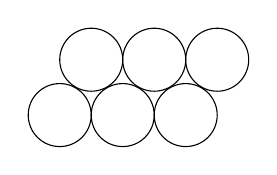
\begin{tikzpicture}[scale=0.8]				
\draw (2,2) circle (0.5cm);
\draw (3,2) circle (0.5cm);
\draw (4,2) circle (0.5cm);
\draw (2.5,1.1213) circle (0.5cm);
\draw (1.5,1.1213) circle (0.5cm);
\draw (3.5,1.1213) circle (0.5cm);
\end{tikzpicture}

B: 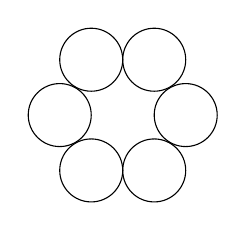
\begin{tikzpicture}[scale=0.8]				
\draw (2,2) circle (0.5cm);
\draw (3,2) circle (0.5cm);
\draw (1.5,1.1213) circle (0.5cm);
\draw (3.5,1.1213) circle (0.5cm);
\draw (2,0.2426) circle (0.5cm);
\draw (3,0.2426) circle (0.5cm);
\end{tikzpicture}

Najpomembnejše: kako s tikzom risati grafe. 

Lahko si že takoj za begin{document} definiramo stil za vozlišča, ni pa treba. Tole je ok, ampak je problematično, če želimo tudi kakšno oznako narisati kot vozlišče:
\begin{verbatim}
% Define style for nodes
\tikzstyle{every node}=[circle, draw, fill=black!10,
inner sep=0pt, minimum width=4pt]
\end{verbatim}

Opomba: meni je všeč, če so vozlišča notri rahlo siva. To je stvar osebnega okusa. Mislim, da ima velika večina ljudi raje notri povsem belo, tako da je morada bolje, da generičen stil nastaviš tako. Da ne bo imel Klavžar težav, ker mu bodo vsi risali v tem stilu ;)


Bolje je nekaj takega:
\begin{verbatim}
\tikzstyle{noeud}=[circle,inner sep=2, minimum size =3 pt, line width = 1pt, draw=black, fill=white]
\end{verbatim}


Lahko pa stil definiramo tudi pri vsaki sliki posebej (primer tega je spodaj).

\begin{figure}[!ht]
	\begin{center}
		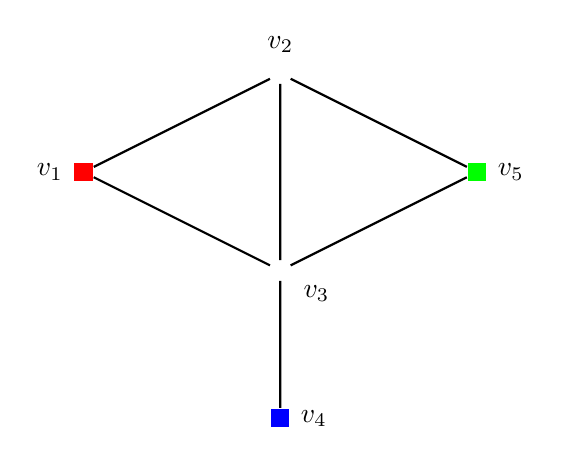
\begin{tikzpicture}[thick,scale=2.5]
		\draw (1,0.5) node[label=left: $v_1$, fill=red](v1) {};
		\draw (2,1) node[label=above: $v_2$](v2) {};
		\draw (2,0) node[label={[label distance=1pt]340:$v_3$}](v3) {};
		\draw (2,-0.75) node[label=right: $v_4$, fill=blue](v4) {};
		\draw (3,0.5) node[label=right: $v_5$, fill=green](v5) {};
		\path[draw] (v1) -- (v2);
		\path[draw] (v2) -- (v5);
		\path[draw] (v1) -- (v3);
		\path[draw] (v3) -- (v5);
		\path[draw] (v2) -- (v3);
		\path[draw] (v3) -- (v4);
		\end{tikzpicture}
		\caption{Graf $G$. Vozlišča lahko tudi obarvamo in označimo. Pri oznakah lahko sami določimo kje bo oznaka (levo, desno, oddaljenost, kot).}
		\label{grafG}
	\end{center}
\end{figure}

\begin{figure}[!ht]
	\begin{center}
		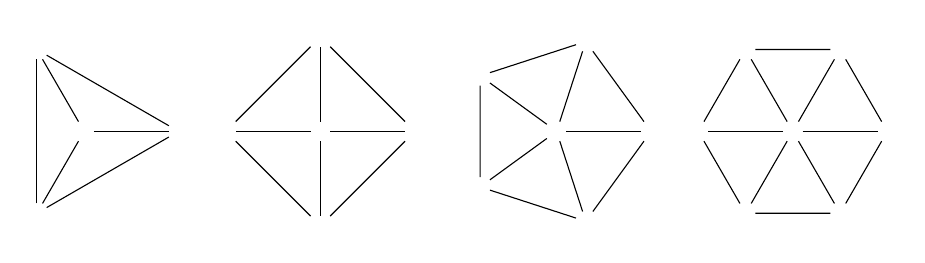
\begin{tikzpicture}[scale=0.6]
		\pgfmathtruncatemacro{\a}{3}
		\pgfmathtruncatemacro{\b}{4}
		\pgfmathtruncatemacro{\c}{5}
		\pgfmathtruncatemacro{\d}{6}
		\pgfmathtruncatemacro{\r}{2}
		\begin{scope}
		\node (c) at (0,0) {};
		\foreach \x in {1,...,\a}
		\node (\x) at (\x*360/\a:\r cm) {};
		\foreach \x [remember=\x as \lastx (initially 1)] in {1,...,\a,1}
		\path (\x) edge (\lastx);
		\foreach \x in {1,...,\a}
		\path (c) edge (\x);
		\end{scope}
		
		\begin{scope}[xshift=5cm]
		\node (c) at (0,0) {};
		\foreach \x in {1,...,\b}
		\node (\x) at (\x*360/\b:\r cm) {};
		\foreach \x [remember=\x as \lastx (initially 1)] in {1,...,\b,1}
		\path (\x) edge (\lastx);
		\foreach \x in {1,...,\b}
		\path (c) edge (\x);
		\end{scope}
		
		\begin{scope}[xshift=10cm]
		\node (c) at (0,0) {};
		\foreach \x in {1,...,\c}
		\node (\x) at (\x*360/\c:\r cm) {};
		\foreach \x [remember=\x as \lastx (initially 1)] in {1,...,\c,1}
		\path (\x) edge (\lastx);
		\foreach \x in {1,...,\c}
		\path (c) edge (\x);
		\end{scope}
		
		\begin{scope}[xshift=15cm]
		\node (c) at (0,0) {};
		\foreach \x in {1,...,\d}
		\node (\x) at (\x*360/\d:\r cm) {};
		\foreach \x [remember=\x as \lastx (initially 1)] in {1,...,\d,1}
		\path (\x) edge (\lastx);
		\foreach \x in {1,...,\d}
		\path (c) edge (\x);
		\end{scope}
		
		\end{tikzpicture}
		\caption{Grafi koles $W_3, W_4, W_5$ in $W_6$. Koordinate točk lahko podamo tudi s polarnimi koordinatami - kulsko. Zelo uporabna zadeva je for zanka, ker je potem manj pisanja. Razložim več (predvsem zale lastx)?}
		\label{malaKolesa}
	\end{center}
\end{figure}

\begin{figure}[!ht]
	\begin{center}
		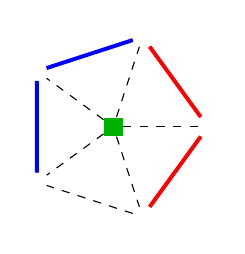
\begin{tikzpicture}[scale=0.6]
		\pgfmathtruncatemacro{\a}{3}
		\pgfmathtruncatemacro{\b}{4}
		\pgfmathtruncatemacro{\c}{5}
		\pgfmathtruncatemacro{\r}{2}
		\node[fill=black!30!green, minimum size = 5pt] (c) at (0,0) {};
		\foreach \x in {1,...,\c}
		\node (\x) at (\x*360/\c:\r cm) {};
		\foreach \x [remember=\x as \lastx (initially 1)] in {1,...,\c,1}
		\path[dashed] (\x) edge (\lastx);
		\foreach \x in {1,...,\c}
		\path[dashed] (c) edge (\x);
		\path[blue, line width=0.5mm] (1) edge (2);
		\path[blue, line width=0.5mm] (2) edge (3);
		\path[red, line width=0.5mm] (1) edge (5);
		\path[red, line width=0.5mm] (5) edge (4);
		\end{tikzpicture}
		\caption{Tudi s črtami lahko delamo marsikaj.}
		\label{malaKolesaIp}
	\end{center}
\end{figure}

Mimogrede, povezavo med $x$ in $y$ lahko narišemo na več načinov: $\backslash$ path (x) edge (y); ali $\backslash$ draw (x) edge (y); ali $\backslash$ draw (x) -- (y); (tu vmes sta dva minusa). Seveda lahko narišemo tudi ukrivljeno povezavo: $\backslash$ draw [bend left=20,-] (x) to (y);

\begin{figure}[!ht]
	\begin{center}
		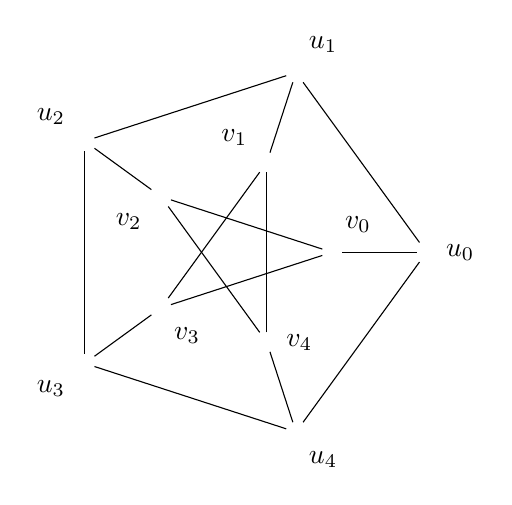
\begin{tikzpicture}[scale=0.6]
		\pgfmathtruncatemacro{\N}{5}
		\pgfmathtruncatemacro{\Nr}{4}
		\pgfmathtruncatemacro{\r}{2}
		\pgfmathtruncatemacro{\R}{4}
		\begin{scope}
		\foreach \x in {0,...,\Nr}
		\node[label={\x*360/\N:$u_{\x}$}] (\x) at (\x*360/\N:\R cm) {};
		\foreach \x [remember=\x as \lastx (initially 0)] in {0,...,\Nr,0}
		\path (\x) edge (\lastx);
		\end{scope}
		
		\begin{scope}
		\foreach \x in {0,...,\Nr}
		\node[label={(\x+1)*360/\N:$v_{\x}$}] (\x+5) at (\x*360/\N:\r cm) {};
		\end{scope}
		
		
		\draw (0+5) edge (2+5); 
		\path (2+5) edge (4+5); 
		\path (4+5) edge (1+5); 
		\path (1+5) edge (3+5); 
		\path (3+5) edge (0+5);
		
		\foreach \x  in {0,...,\Nr}
		\path (\x) edge (\x+5);
		
		\end{tikzpicture}
		\caption{Petersenov graf.}
		\label{petersen}
	\end{center}
\end{figure}

\begin{figure}[!ht]
	\begin{center}
		
\begin{tikzpicture}
		\pgfmathtruncatemacro{\m}{6}
		\pgfmathtruncatemacro{\n}{4}
		\begin{scope}
		\foreach \x in {1,...,\m}
		\foreach \y in {1,...,\n}
		\node (\x,\y) at (\x, \y) {};
		\foreach \x [remember=\x as \lastx (initially 1)] in {1,...,\m}
		\foreach \y in {1,...,\n}
		\path (\x, \y) edge (\lastx, \y);
		
		\foreach \y [remember=\y as \lasty (initially 1)] in {1,...,\n}
		\foreach \x in {1,...,\m}
		\path (\x, \y) edge (\x, \lasty);
		\foreach \x in {1,...,\m}
		\foreach \y in {1,...,\n}
		\node (\x,\y) at (\x, \y) {};
		\end{scope}
		\end{tikzpicture}
		\caption{Graf $P_6 \square P_4$ (mreža).}
		\label{grafmreza}
	\end{center}
\end{figure}

Prikazan še drug stil vozlišč (z nekoliko neposrečenim imenom, morda ga raje spremeni). Tu je stil definiran znotraj slike. Tudi stil za node je popravljen, sicer oznake niso lepo narisane (ampak so v sivih krogcih). Za tole je treba dodati še paketek decorations.pathreplacing, da imaš tiste lepe zavite zaklepaje zgoraj. Mogoče je ta primer že preveč zapleten in raje drugačen stil za vozlišča pokaži na enem od zgornjih lažjih primerov.

\begin{figure}[ht!]
	\begin{center}
		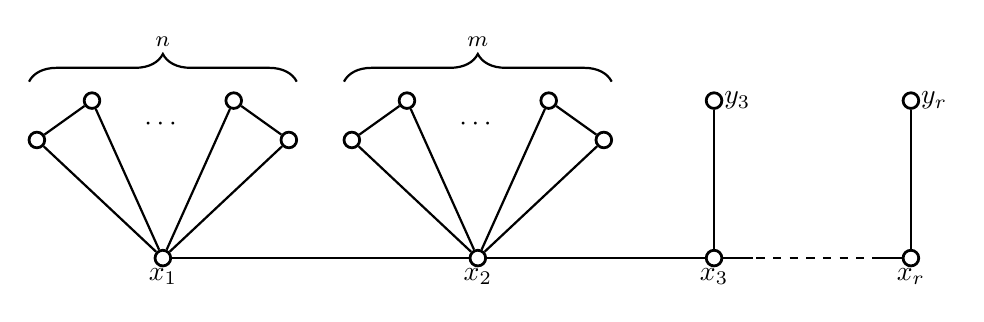
\begin{tikzpicture}[scale=1.0,style=thick,x=1cm,y=1cm]
		\def\vr{3pt}
		
		\tikzstyle{noeud}=[circle,inner sep=2, minimum size =3 pt, line width = 1pt, draw=black, fill=white]
		\tikzstyle{every node}=[]
		
		% vertices
		
		\node[noeud] (x1) at (0,0){};
		\node[noeud] (x2) at (4,0){};
		\node[noeud] (x3) at (7,0){};
		\node[noeud] (xr) at (9.5,0){};
		\node[noeud] (x3') at (7,2){};
		\node[noeud] (xr') at (9.5,2){};
		\node[noeud] (y1) at (-1.6,1.5){};
		\node[noeud] (y1') at (-0.9,2){};
		\node[noeud] (yt-k-1) at (0.9,2){};
		\node[noeud] (yt-k-1') at (1.6,1.5){};
		\node[noeud] (z1) at (2.4,1.5){};
		\node[noeud] (z1') at (3.1,2){};
		\node[noeud] (zt-k-1) at (4.9,2){};
		\node[noeud] (zt-k-1') at (5.6,1.5){};
		
		% edges
		\draw (x1) -- (x2) -- (x3);
		\draw (x1) -- (y1) -- (y1') -- (x1);
		\draw (x1) -- (yt-k-1) -- (yt-k-1') -- (x1);
		\draw (x2) -- (z1) -- (z1') -- (x2);
		\draw (x2) -- (zt-k-1) -- (zt-k-1') -- (x2);
		\draw (x3) -- (7.5,0);
		\draw[dashed] (x3) -- (xr);
		\draw (xr) -- (9,0);
		\draw (x3) -- (x3');
		\draw (xr) -- (xr');
		
		
		% labels
		
		\draw [decorate,decoration={brace,amplitude=10pt,raise=4pt}] (-1.7,2.1)-- (1.7,2.1)node[above= 13pt,midway]{\footnotesize $n$};
		\draw [decorate,decoration={brace,amplitude=10pt,raise=4pt}] (2.3,2.1)-- (5.7,2.1)node[above= 13pt,midway]{\footnotesize $m$};
		\draw (0,1.7) node {$\cdots$};
		\draw (4,1.7) node {$\cdots$};
		\draw(x1) node[below] {$x_{1}$};
		\draw(x2) node[below] {$x_{2}$};
		\draw(x3) node[below] {$x_{3}$};
		\draw(xr) node[below] {$x_{r}$};
		\draw(x3') node[right] {$y_{3}$};
		\draw(xr') node[right] {$y_{r}$};
		
		\end{tikzpicture}
	\end{center}
	\caption{En lep graf.}
	\label{fig:Grst}
\end{figure}


\end{document}
% vim: syntax=tex
% vim: spell spelllang=sl
% vim: foldlevel=99
% Latex template: Jure Slak, jure.slak@gmail.com

